\begin{figure}[!h]
\centering
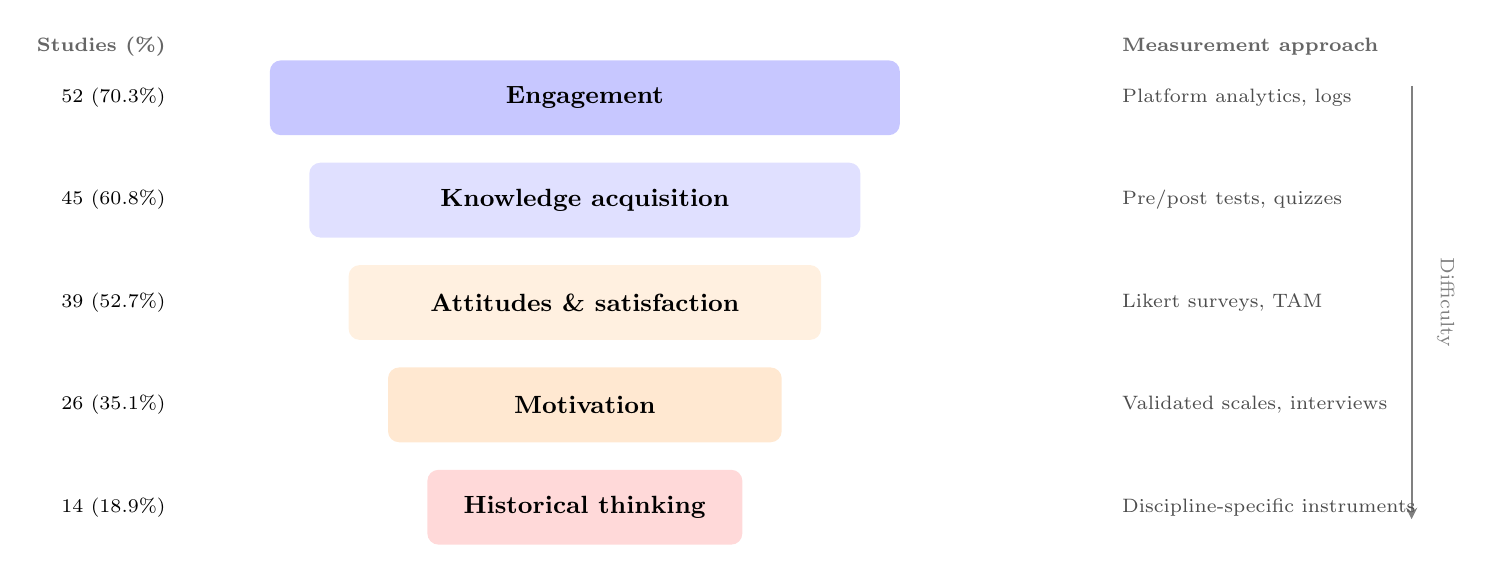
\begin{tikzpicture}[
    every node/.style={font=\small},
    level/.style={
        rounded corners=4pt,
        minimum height=0.95cm,
        text=black,
        align=center,
        anchor=center,
    }
]

% Vertical spacing between levels
\def\yspacing{1.30}

% Level widths (progressively narrower)
\def\wA{8.0}   % Engagement
\def\wB{7.0}   % Knowledge
\def\wC{6.0}   % Attitudes
\def\wD{5.0}   % Motivation
\def\wE{4.0}   % Historical thinking

% Fixed annotation positions
\def\chartcenter{-1.5}  % shift bars left
\def\leftcol{-6.7}
\def\rightcol{5.2}

% Y positions (top to bottom)
\def\yA{0}
\pgfmathsetmacro{\yB}{\yA - \yspacing}
\pgfmathsetmacro{\yC}{\yB - \yspacing}
\pgfmathsetmacro{\yD}{\yC - \yspacing}
\pgfmathsetmacro{\yE}{\yD - \yspacing}

% --- Column headers ---
\node[font=\scriptsize\bfseries, anchor=east, text=black!60] at (\leftcol, 0.65)
    {Studies (\%)};
\node[font=\scriptsize\bfseries, anchor=west, text=black!60] at (\rightcol, 0.65)
    {Measurement approach};

% --- Downward arrow (right margin, compact) ---
\draw[-stealth, thick, black!50] (\rightcol + 3.8, \yA + 0.15) -- (\rightcol + 3.8, \yE - 0.15);
\node[rotate=-90, anchor=south, font=\scriptsize, text=black!50] at (\rightcol + 4.0, {(\yA + \yE)/2})
    {Difficulty};

% --- Level 1: Engagement ---
\node[level, fill=blue!22, minimum width=\wA cm] (L1) at (\chartcenter, \yA)
    {\textbf{Engagement}};
\node[anchor=east, font=\scriptsize] at (\leftcol, \yA)
    {52 (70.3\%)};
\node[anchor=west, font=\scriptsize, text=black!70] at (\rightcol, \yA)
    {Platform analytics, logs};

% --- Level 2: Knowledge acquisition ---
\node[level, fill=blue!12, minimum width=\wB cm] (L2) at (\chartcenter, \yB)
    {\textbf{Knowledge acquisition}};
\node[anchor=east, font=\scriptsize] at (\leftcol, \yB)
    {45 (60.8\%)};
\node[anchor=west, font=\scriptsize, text=black!70] at (\rightcol, \yB)
    {Pre/post tests, quizzes};

% --- Level 3: Attitudes & satisfaction ---
\node[level, fill=orange!12, minimum width=\wC cm] (L3) at (\chartcenter, \yC)
    {\textbf{Attitudes \& satisfaction}};
\node[anchor=east, font=\scriptsize] at (\leftcol, \yC)
    {39 (52.7\%)};
\node[anchor=west, font=\scriptsize, text=black!70] at (\rightcol, \yC)
    {Likert surveys, TAM};

% --- Level 4: Motivation ---
\node[level, fill=orange!18, minimum width=\wD cm] (L4) at (\chartcenter, \yD)
    {\textbf{Motivation}};
\node[anchor=east, font=\scriptsize] at (\leftcol, \yD)
    {26 (35.1\%)};
\node[anchor=west, font=\scriptsize, text=black!70] at (\rightcol, \yD)
    {Validated scales, interviews};

% --- Level 5: Historical thinking ---
\node[level, fill=red!15, minimum width=\wE cm] (L5) at (\chartcenter, \yE)
    {\textbf{Historical thinking}};
\node[anchor=east, font=\scriptsize] at (\leftcol, \yE)
    {14 (18.9\%)};
\node[anchor=west, font=\scriptsize, text=black!70] at (\rightcol, \yE)
    {Discipline-specific instruments};

\end{tikzpicture}
\caption{Ease-of-measurement hierarchy for gamification outcome types. Outcome frequency inversely correlates with measurement difficulty: the evidence base is dominated by easy-to-measure outcomes (engagement, knowledge) while discipline-specific outcomes (historical thinking) remain underrepresented.}
\label{fig:outcome-taxonomy}
\end{figure}
